\documentclass[fullscreen=true, unicode, bookmarks=false]{beamer}
\usepackage[T2A]{fontenc}
\usepackage[utf8]{inputenc}
\usepackage[english, russian]{babel}
\usepackage{amsmath}
\usepackage{amsmath,amsfonts,amssymb}
\usepackage[export]{adjustbox}
\usepackage{textgreek}
\newtheorem{rustheorem}{Теорема }
\sloppy

\DeclareMathOperator{\arsh}{arsh}

\setbeamertemplate{navigation symbols}{}

\usetheme{Madrid}

\usecolortheme{whale}

\usefonttheme{professionalfonts} % default family is serif

\setbeamertemplate{footline}{\hspace*{.5cm}\scriptsize{\insertshorttitle
\hspace*{50pt} \hfill\hspace*{.5cm}}\vspace{5pt}} 

\setbeamercolor{bibliography entry author}{fg=black}

\title[]{ {\huge Dynamics of diffused connected systems of differential equations with internal connection } }   
\author[]{{\large Leonid Ivanovsky}} 
\date{ }
\institute[]
{ P.G. Demidov Yaroslavl State University }

\begin{document}

\begin{frame}
\titlepage
\end{frame} 

\begin{frame}
\frametitle{ Diffused connected system of differential equations }
 
\begin{equation}
	\dot u_j = N^2(u_{j+1} - 2u_j + u_{j-1}) + \gamma u_j, \qquad j = \overline{1, N},
\end{equation}

\begin{equation}
	u_0 = u_1, \quad u_{N+1} = u_N + \dfrac{\alpha}{N}u_k + \dfrac{\beta}{N}u_k^3, \qquad 1 \le k < N,
\end{equation}

\bigskip

$$ u_j = u_j(t), \quad t \geqslant 0, \quad \alpha, \beta, \gamma \in \mathbb{R}. $$

\end{frame}

\begin{frame}
\frametitle{ Linearized system of differential equations }
 
\begin{equation}
	\dot u_j = N^2(u_{j+1} - 2u_j + u_{j-1}) + \gamma u_j, \qquad j = \overline{1, N},
\end{equation}

\bigskip

\begin{equation}
	u_0 = u_1, \quad u_{N+1} = u_N + \dfrac{\alpha}{N}u_k, \qquad 1 \leqslant k < N,
\end{equation}

\end{frame}

\begin{frame}
\frametitle{ Eigenvalue problem }
 
$$ u_j = e^{\lambda t} \ch \delta x_j, $$

$$ x_j = -\dfrac{1}{2N} + \dfrac{j}{N}. $$

\bigskip
\pause

\begin{itemize}

\item { $ j \leqslant N-1: $ 
}
\begin{equation}
\delta = 2N \arsh \dfrac{\sqrt{-\gamma+\lambda}}{2N}.
\end{equation}
\medskip
\pause
\item { $ j = N: $ 
}
\begin{equation}
\alpha = \dfrac{\sqrt{-\gamma+\lambda}\sh\delta}{\ch\delta x_k}.
\end{equation}

\end{itemize}

\end{frame}

\begin{frame}
\frametitle{ Stability loss of zero solution }

\begin{itemize}

\item { $ \lambda = 0: $ 
}

$$ \alpha_u = \frac{ \sqrt{-\gamma} \, \sh \delta_u }{ \ch\delta_u x_k }, \qquad \delta_u = 2N \arsh \dfrac{\sqrt{-\gamma}}{2N}. $$

\medskip
\pause

\item { $ \lambda = \pm i \omega: \; $ 
}

$$ \alpha_c = \frac{ \sqrt{-\gamma + i \omega} \, \sh \delta_c }{ \ch\delta_c x_k }, \qquad \delta_c = 2N \arsh \dfrac{\sqrt{-\gamma + i \omega}}{2N}. $$

\end{itemize}

\bigskip
\pause

$$ N = 50. $$	

\end{frame}

\begin{frame}
\frametitle{ Extreme case }

$$ N \rightarrow \infty: \qquad \delta \rightarrow \sqrt{-\gamma + \lambda}. $$

\bigskip
\pause

\begin{equation}
	\dot u = u'' + \gamma u,	
\end{equation}
\begin{equation}
	u'(0, t) \, = 0, \qquad u'(1, t) \, = \alpha\,u(x_0, t) + \beta u^3(x_0, t),
\end{equation}

\smallskip

$$ x \in [0,1] ,\quad  x_0 \in [0, 1). $$

\bigskip
\pause

\begin{equation}
\alpha = \dfrac{\sqrt{-\gamma+\lambda}\sh\sqrt{-\gamma+\lambda}}{\ch\sqrt{-\gamma+\lambda}\:x_0}.
\end{equation}

\end{frame}

\begin{frame}
\frametitle{ Visualization of critical dependencies $ \alpha_{cr}(\gamma), \; 1 \leqslant k \leqslant 17 $ }

\begin{figure} 
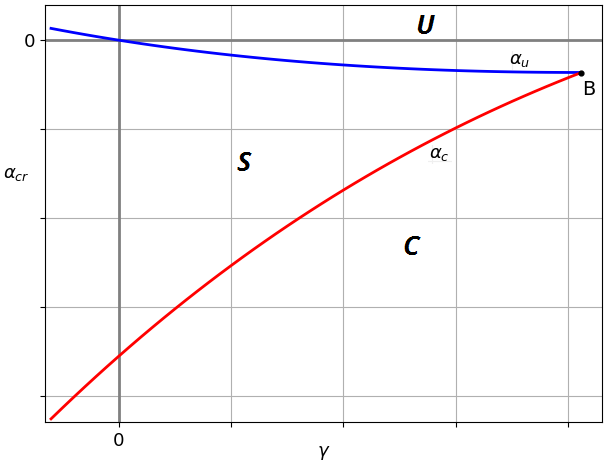
\includegraphics[scale=0.59]{scheme0117.png}  
\end{figure}
$$ B=(\gamma_*, \alpha_*) $$

\end{frame}

\begin{frame}
\frametitle{ Plot $ \alpha_{cr}(\gamma), \; k = 1 $ }

\begin{figure} 
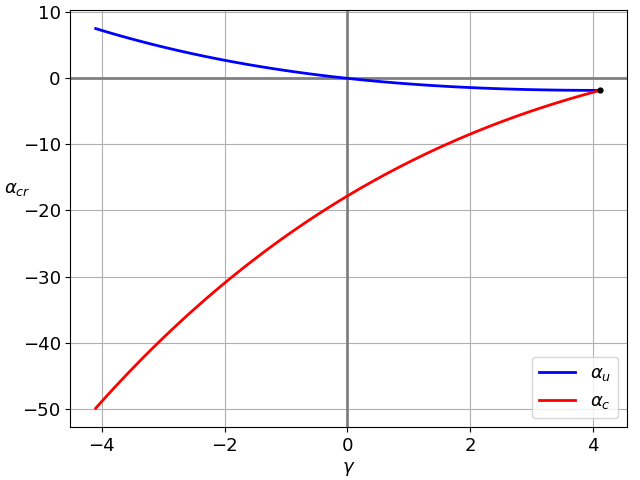
\includegraphics[scale=0.55]{alphas_000.png}  
\end{figure}
$$ \gamma_* \approx 4.116 $$

\end{frame}

\begin{frame}
\frametitle{ Plot $ \alpha_{cr}(\gamma), \; k = 17 $ }

\begin{figure} 
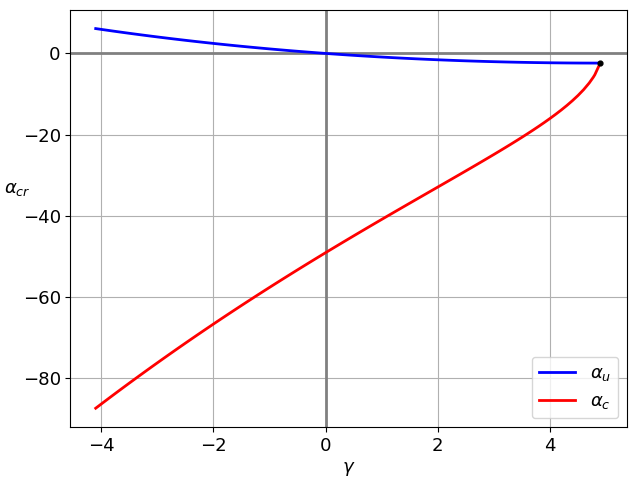
\includegraphics[scale=0.55]{alphas_033.png}  
\end{figure}
$$ \gamma_* \approx 4.896 $$

\end{frame}

\begin{frame}
\frametitle{ Visualization of critical dependencies $ \alpha_{cr}(\gamma), \; 18 \leqslant k \leqslant 23 $ }

\begin{figure} 
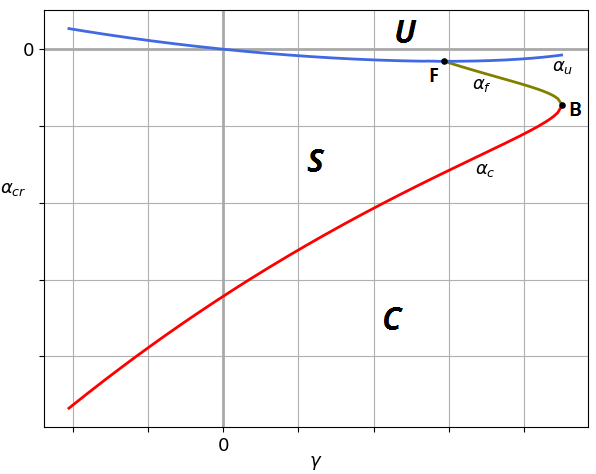
\includegraphics[scale=0.59]{scheme1823.png}  
\end{figure}
$$ F = (\overline{\gamma}, \overline{\alpha}) $$

\end{frame}

\begin{frame}
\frametitle{ Plot $ \alpha_{cr}(\gamma), \; k = 20 $ }

\begin{figure} 
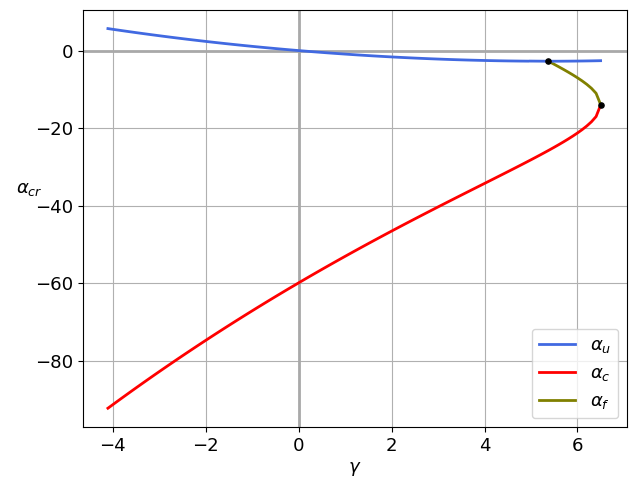
\includegraphics[scale=0.55]{alphas_039.png}  
\end{figure}
$$ \overline{\gamma} \approx 5.375, \; \gamma_* \approx 6.497 $$

\end{frame}

\begin{frame}
\frametitle{ Plot $ \alpha_{cr}(\gamma), \; k = 23 $ }

\begin{figure} 
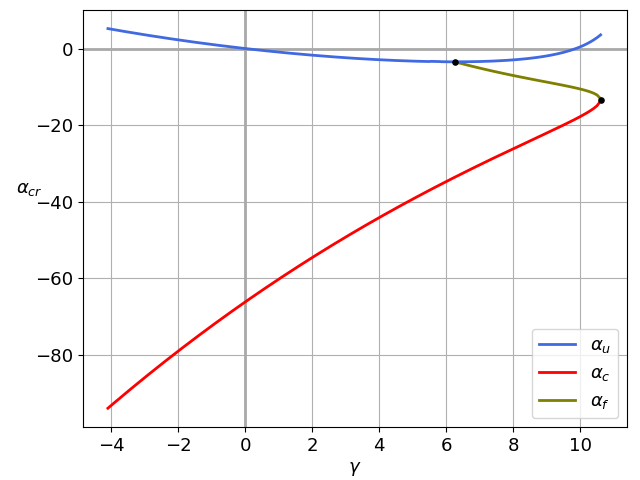
\includegraphics[scale=0.55]{alphas_045.png}  
\end{figure}
$$ \overline{\gamma} \approx 6.258, \; \gamma_* \approx 10.608 $$

\end{frame}

\begin{frame}
\frametitle{ Plot $ \alpha_{cr}(\gamma), \; k = 24 $ }

\begin{figure} 
\begin{minipage}[h]{0.49\linewidth}
\begin{center}
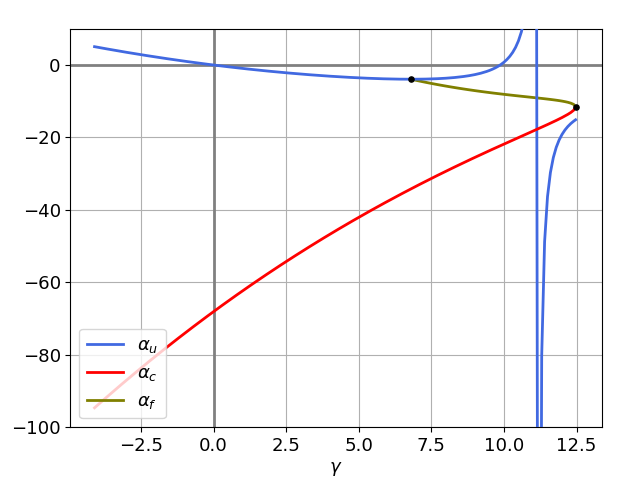
\includegraphics[scale=0.37]{alphas_047.png} 
\end{center}
\end{minipage} 
\hfill
\begin{minipage}[h]{0.49\linewidth}
\begin{center}
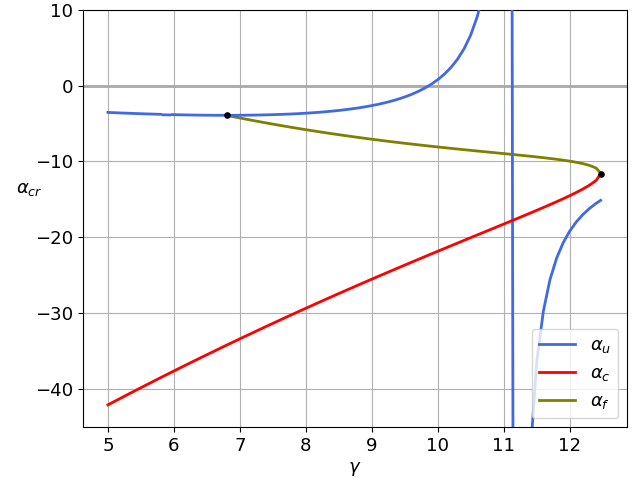
\includegraphics[scale=0.37]{alphas_intersection_047.png}
\end{center}
\end{minipage} 
\end{figure}

$$ \overline{\gamma} \approx 6.798, \; \gamma_* \approx 12.467 $$

\end{frame}

\begin{frame}
\frametitle{ Plot $ \alpha_{cr}(\gamma), \; k = 25 $ }

\begin{figure} 
\begin{minipage}[h]{0.49\linewidth}
\begin{center}
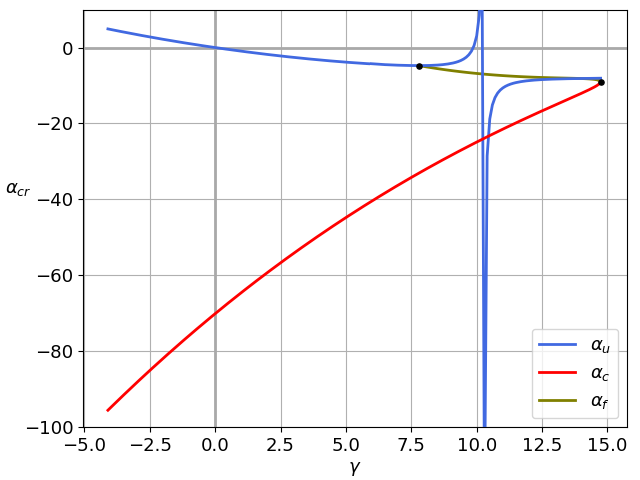
\includegraphics[scale=0.37]{alphas_049.png} 
\end{center}
\end{minipage} 
\hfill
\begin{minipage}[h]{0.49\linewidth}
\begin{center}
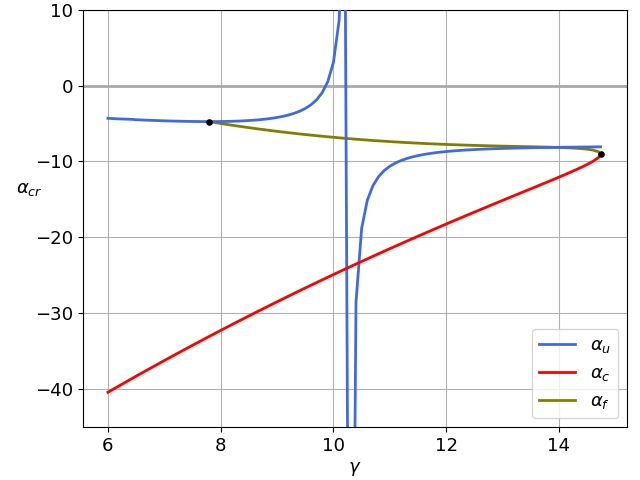
\includegraphics[scale=0.37]{alphas_intersection_049.png}
\end{center}
\end{minipage} 
\end{figure}

$$ \overline{\gamma} \approx 7.794, \; \gamma_* \approx 14.738 $$

\end{frame}

\begin{frame}
\frametitle{ Visualization of critical dependencies $ \alpha_{cr}(\gamma), \; 26 \leqslant k \leqslant 50 $ }

\begin{figure} 
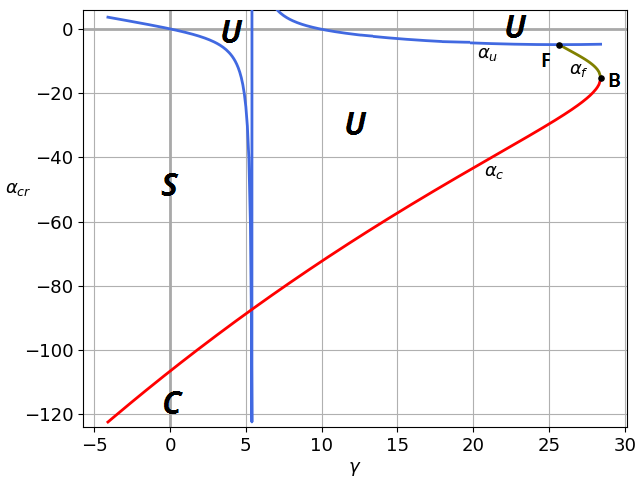
\includegraphics[scale=0.59]{scheme2650.png}  
\end{figure}

\end{frame}

\begin{frame}
\frametitle{ Plot $ \alpha_{cr}(\gamma), \; k = 33 $ }

\begin{figure} 
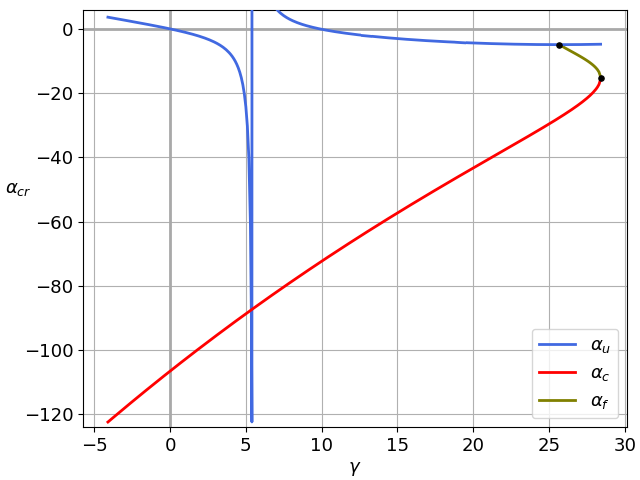
\includegraphics[scale=0.55]{alphas_067.png}  
\end{figure}
$$ \overline{\gamma} \approx 25.682, \; \gamma_* \approx 28.407 $$

\end{frame}

\begin{frame}
\frametitle{ Local analysis }

\begin{equation}
	u_j = \sqrt{\varepsilon}u_{j,0} + \varepsilon u_{j,1} + \varepsilon^{\frac{3}{2}} u_{j,2} + O(\varepsilon^2), \qquad j = \overline{1, N}
\end{equation}

\bigskip

$$ u_j = u_j(s), \quad s = \varepsilon t, $$

$$ \varepsilon = | \alpha - \alpha_{cr} |, \quad \varepsilon \ll 1.  $$

\end{frame}

\begin{frame}
\frametitle{ Divergent case of stability loss }

\begin{itemize}
\item { $ \lambda = 0: \quad \varepsilon=\alpha-\alpha_u, $
}
\end{itemize}

\bigskip

\begin{equation}
	\dot u_{j,0} = N^2(u_{j+1,0} - 2u_{j,0} + u_{j-1,0}) + \gamma u_{j,0},
\end{equation}
\begin{equation}
	u_{0,0} = u_{1,0}, \quad u_{N+1,0} = u_{N,0} + \dfrac{\alpha}{N}u_{k,0},
\end{equation}

\bigskip

$$ u_{j,0} = \rho(s) \ch \delta_u x_j, $$

$$ \delta_u = 2N \arsh \dfrac{\sqrt{-\gamma}}{2N}, \quad x_j = -\dfrac{1}{2N} + \dfrac{j}{N}. $$

\end{frame}

\begin{frame}
\frametitle{ Divergent case of stability loss }

\begin{equation}
	\dot u_{j,2} + \frac{\partial u_{j,0}}{\partial s} = N^2(u_{j+1,2} - 2u_{j,2} + u_{j-1,2}) + \gamma u_{j,2},
\end{equation}
\begin{equation}
	u_{0,2} = u_{1,2}, \quad u_{N+1,2} = u_{N,2} + \dfrac{\alpha}{N}u_{k,0} + \dfrac{\beta}{N}u_{k,0}, \qquad 1 \le k < N,
\end{equation}

\bigskip

$$ u_{j,2} = \ch \delta_u x_j. $$


\end{frame}

\begin{frame}
\frametitle{ Divergent case of stability loss }

\begin{equation}
	\rho' = \phi_0 \rho + d_0 \rho^3,
\end{equation}

\bigskip

$$ \phi_0 = Q \ch \delta_u x_k, \qquad d_0 = \beta Q \ch^3 \delta_u x_k, $$

\bigskip

$$ Q = \frac{2 \delta_u}{\delta_u\ch \delta_u + \sh \delta_u - \alpha_u x_k \sh \delta_u x_k}, $$

$$ \alpha_u = \frac{ \sqrt{-\gamma} \, \sh \delta_u }{ \ch\delta_u x_k }. $$

\end{frame}

\begin{frame}
\frametitle{ Plot $ \phi_0(\gamma) $ and $ d_0(\gamma), \; k = 1 $ }

\begin{figure} 
\begin{minipage}[h]{0.49\linewidth}
\begin{center}
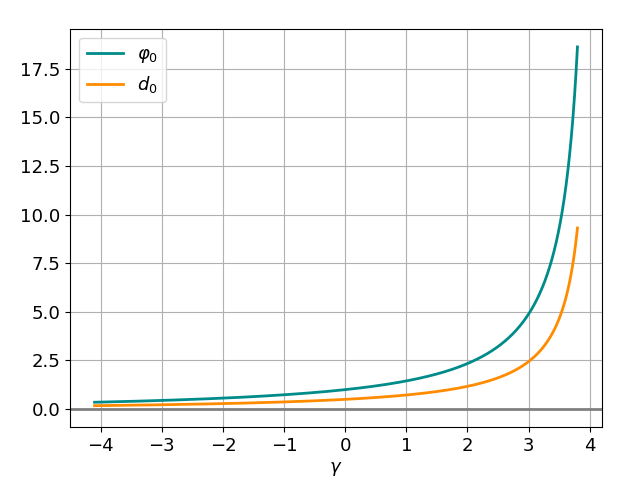
\includegraphics[scale=0.39]{divergent_phid_x0_000_beta_05.png} \\ {\scriptsize a) $ \beta = 0.5 $}
\end{center}
\end{minipage} 
\hfill
\begin{minipage}[h]{0.49\linewidth}
\begin{center}
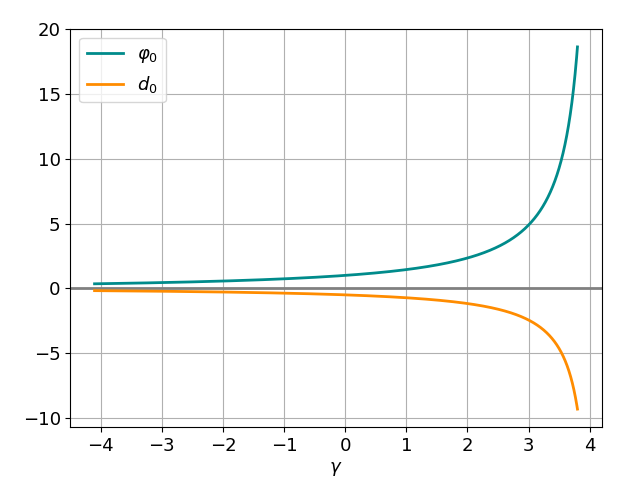
\includegraphics[scale=0.39]{divergent_phid_x0_000_beta_-05.png}  \\ {\scriptsize b) $ \beta = -0.5 $}
\end{center}
\end{minipage} 
\end{figure}
$$ \gamma_* \approx 4.116 $$

\end{frame}

\begin{frame}
\frametitle{ Plot $ \phi_0(\gamma) $ and $ d_0(\gamma), \; k = 20 $ }

\begin{figure} 
\begin{minipage}[h]{0.49\linewidth}
\begin{center}
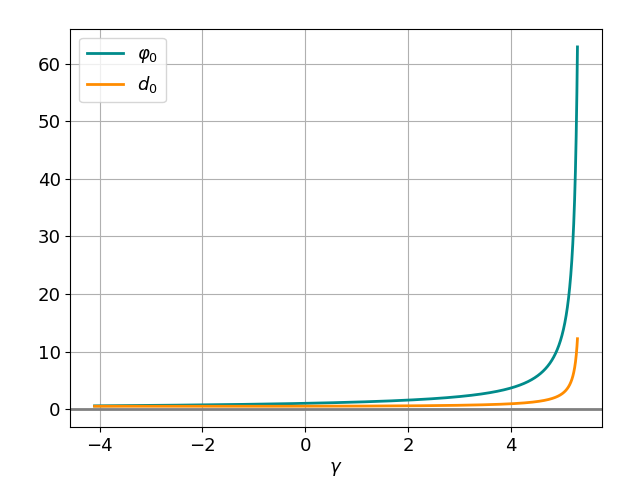
\includegraphics[scale=0.39]{divergent_phid_x0_039_beta_05.png} \\ {\scriptsize a) $ \beta = 0.5 $}
\end{center}
\end{minipage} 
\hfill
\begin{minipage}[h]{0.49\linewidth}
\begin{center}
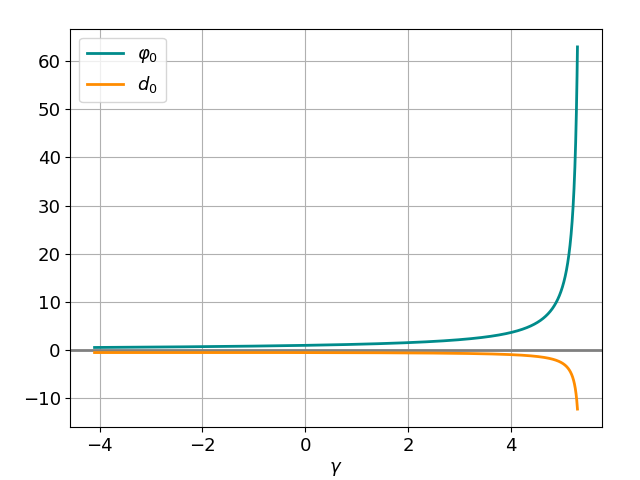
\includegraphics[scale=0.39]{divergent_phid_x0_039_beta_-05.png}  \\ {\scriptsize b) $ \beta = -0.5 $}
\end{center}
\end{minipage} 
\end{figure}
$$ \overline{\gamma} \approx 5.375 $$

\end{frame}

\begin{frame}
\frametitle{ Plot $ \phi_0(\gamma) $ and $ d_0(\gamma), \; k = 20 $ }

\begin{figure} 
\begin{minipage}[h]{0.49\linewidth}
\begin{center}
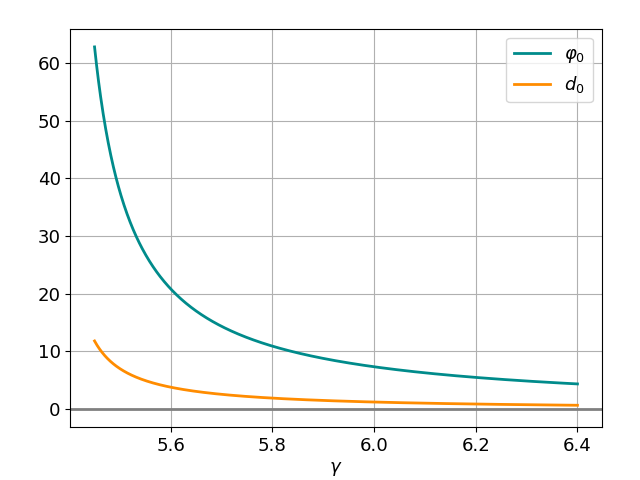
\includegraphics[scale=0.39]{divergent_phid_x0_039_beta_05-1.png} \\ {\scriptsize a) $ \beta = 0.5 $}
\end{center}
\end{minipage} 
\hfill
\begin{minipage}[h]{0.49\linewidth}
\begin{center}
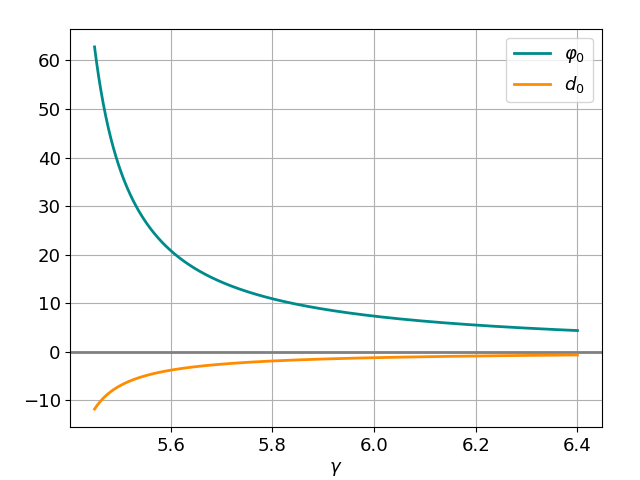
\includegraphics[scale=0.39]{divergent_phid_x0_039_beta_-05-1.png}  \\ {\scriptsize b) $ \beta = -0.5 $}
\end{center}
\end{minipage} 
\end{figure}
$$ \overline{\gamma} \approx 5.375, \; \gamma_* \approx 6.497 $$

\end{frame}

\begin{frame}
\frametitle{ Oscillating case of stability loss }

\begin{itemize}
\item { $ \lambda = \pm i \omega: \quad \varepsilon=\alpha_c-\alpha, $
}
\end{itemize}

\bigskip

\begin{equation}
	\dot u_{j,0} = N^2(u_{j+1,0} - 2u_{j,0} + u_{j-1,0}) + \gamma u_{j,0},
\end{equation}
\begin{equation}
	u_{0,0} = u_{1,0}, \quad u_{N+1,0} = u_{N,0} + \dfrac{\alpha}{N}u_{k,0},
\end{equation}

\bigskip

$$ u_{j,0} = z(s) e^{i \omega t} \ch \delta_c x_j + \overline{z(s)} e^{-i \omega t} \overline{\ch \delta_c x_j}, $$

$$ \delta_c = 2N \arsh \dfrac{\sqrt{-\gamma + i \omega}}{2N}, \quad x_j = -\dfrac{1}{2N} + \dfrac{j}{N}. $$

\end{frame}

\begin{frame}
\frametitle{ Oscillating case of stability loss }

\begin{equation}
	\dot u_{j,2} + \frac{\partial u_{j,0}}{\partial s} = N^2(u_{j+1,2} - 2u_{j,2} + u_{j-1,2}) + \gamma u_{j,2},
\end{equation}
\begin{equation}
	u_{0,2} = u_{1,2}, \quad u_{N+1,2} = u_{N,2} + \dfrac{\alpha}{N}u_{k,0} + \dfrac{\beta}{N}u_{k,0}, \qquad 1 \le k < N,
\end{equation}

\bigskip

$$ u_{j,2} = e^{i \omega t} \ch \delta_c x_j. $$

\end{frame}

\begin{frame}
\frametitle{ Oscillating case of stability loss }

\begin{equation}
	z' = \phi_0 z + d_0 z |z|^2,
\end{equation}

\bigskip

$$ \phi_0 = -\mbox{Re} \left(\dfrac{2 \delta_c \ch \delta_c x_k}{\delta_c\ch \delta_c + \sh \delta_c - \alpha_c x_k \sh \delta_c x_k} \right), $$

$$ d_0 = \mbox{Re} \left( \dfrac{3 \beta \delta_c (\ch \chi x_k + \ch \eta x_k + 2 \ch \overline{\delta_c} x_k)}{2(\delta_c\ch \delta_c + \sh \delta_c - \alpha_c x_k \sh \delta_c x_k)} \right), $$

\bigskip

$$ \chi = \delta_c + 2\mbox{Re}\:\delta_c, \quad \eta = \delta_c + 2i\:\mbox{Im}\:\delta_c, $$

$$ \alpha_c = \frac{ \sqrt{-\gamma + i \omega} \, \sh \delta_c }{ \ch\delta_c x_k }. $$

\end{frame}

\begin{frame}
\frametitle{ Plot $ \phi_0(\gamma) $ and $ d_0(\gamma), \; k = 1 $ }

\begin{figure} 
\begin{minipage}[h]{0.49\linewidth}
\begin{center}
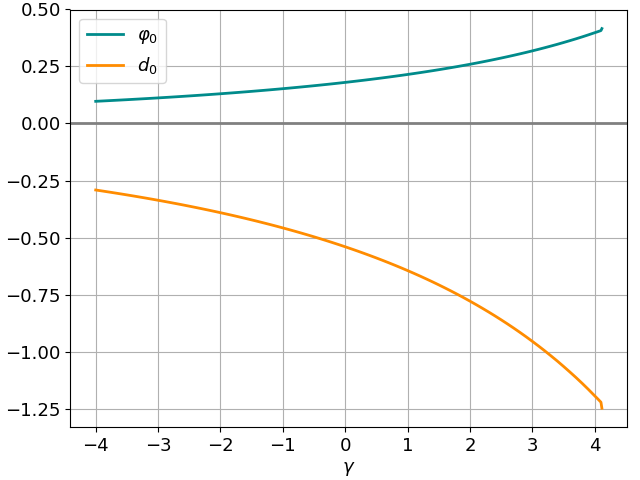
\includegraphics[scale=0.37]{oscillating_phi0d0_x0_000_beta_10.png} \\ {\scriptsize a) $ \beta = 1.0 $}
\end{center}
\end{minipage} 
\hfill
\begin{minipage}[h]{0.49\linewidth}
\begin{center}
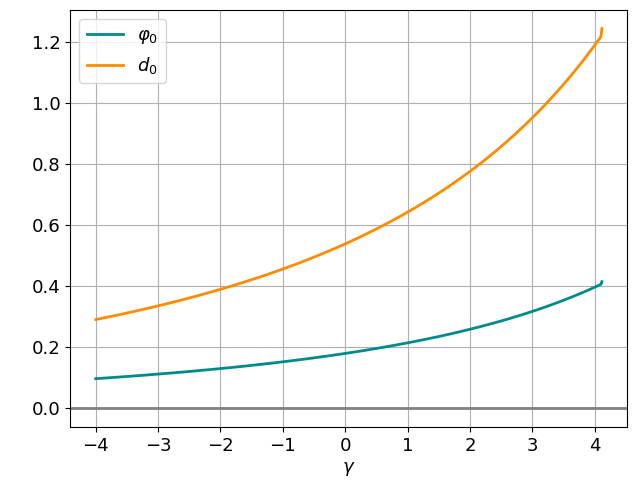
\includegraphics[scale=0.37]{oscillating_phi0d0_x0_000_beta_-10.png}  \\ {\scriptsize b) $ \beta = -1.0 $}
\end{center}
\end{minipage} 
\end{figure}
$$ \gamma_* \approx 4.116 $$

\end{frame}

\begin{frame}
\frametitle{ Plot $ \phi_0(\gamma) $ and $ d_0(\gamma), \; k = 17 $ }

\begin{figure} 
\begin{minipage}[h]{0.49\linewidth}
\begin{center}
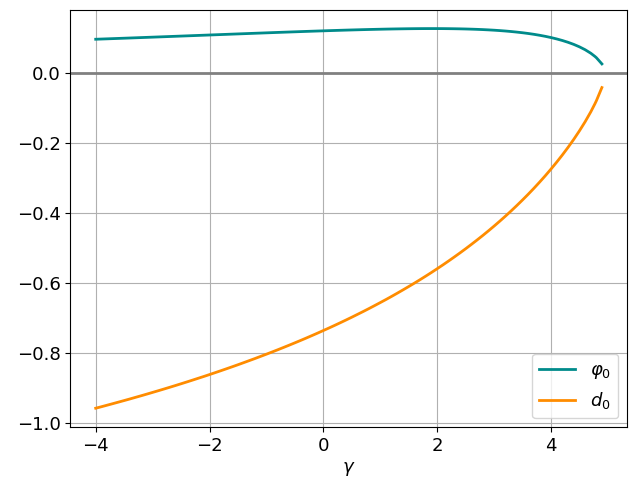
\includegraphics[scale=0.37]{oscillating_phi0d0_x0_033_beta_10.png} \\ {\scriptsize a) $ \beta = 1.0 $}
\end{center}
\end{minipage} 
\hfill
\begin{minipage}[h]{0.49\linewidth}
\begin{center}
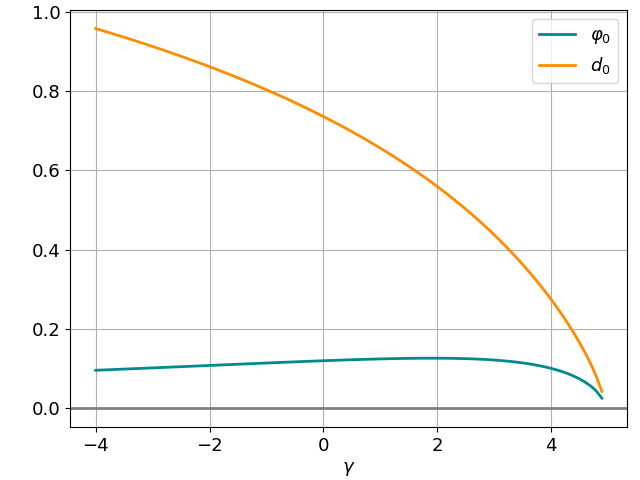
\includegraphics[scale=0.37]{oscillating_phi0d0_x0_033_beta_-10.png}  \\ {\scriptsize b) $ \beta = -1.0 $}
\end{center}
\end{minipage} 
\end{figure}
$$ \gamma_* \approx 4.896 $$

\end{frame}

\begin{frame}
\frametitle{ Plot $ \phi_0(\gamma) $ and $ d_0(\gamma), \; \alpha_{cr} = \alpha_c, k = 20 $ }

\begin{figure} 
\begin{minipage}[h]{0.49\linewidth}
\begin{center}
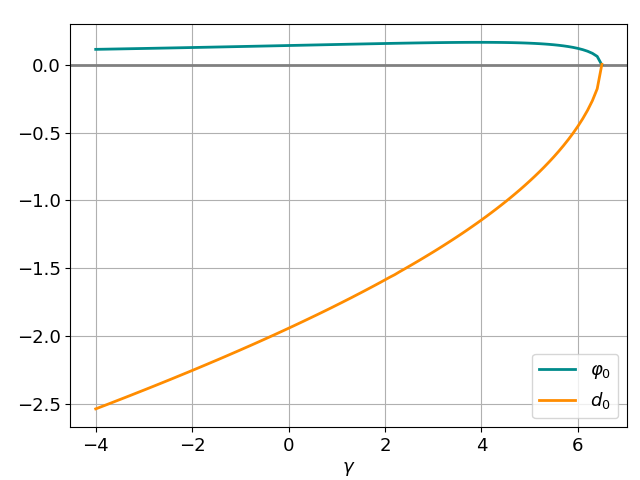
\includegraphics[scale=0.37]{oscillating_phi0d0_x0_039_beta_10.png} \\ {\scriptsize a) $ \beta = 1.0 $}
\end{center}
\end{minipage} 
\hfill
\begin{minipage}[h]{0.49\linewidth}
\begin{center}
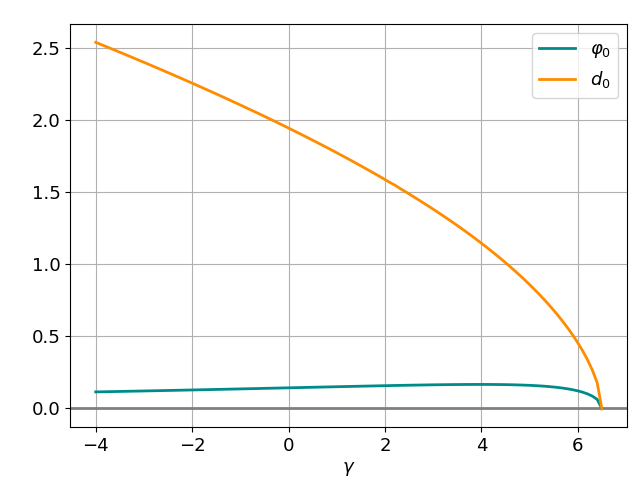
\includegraphics[scale=0.37]{oscillating_phi0d0_x0_039_beta_-10.png}  \\ {\scriptsize b) $ \beta = -1.0 $}
\end{center}
\end{minipage} 
\end{figure}
$$ \gamma_* \approx 6.497 $$

\end{frame}

\begin{frame}
\frametitle{ Plot $ \phi_0(\gamma) $ and $ d_0(\gamma), \; \alpha_{cr} = \alpha_f, k = 20 $ }

\begin{figure} 
\begin{minipage}[h]{0.49\linewidth}
\begin{center}
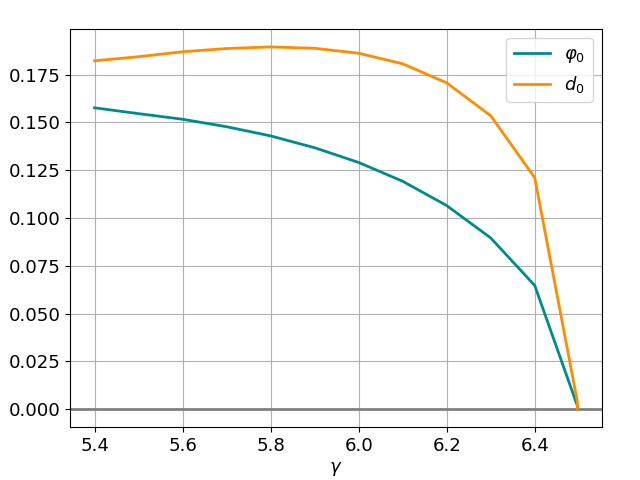
\includegraphics[scale=0.37]{oscillating_phi0d0_after_tangent_x0_039_beta_10.png} \\ {\scriptsize a) $ \beta = 1.0 $}
\end{center}
\end{minipage} 
\hfill
\begin{minipage}[h]{0.49\linewidth}
\begin{center}
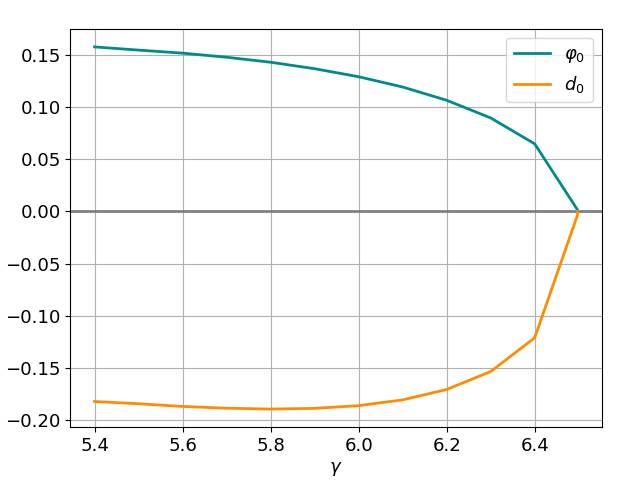
\includegraphics[scale=0.37]{oscillating_phi0d0_after_tangent_x0_039_beta_-10.png}  \\ {\scriptsize b) $ \beta = -1.0 $}
\end{center}
\end{minipage} 
\end{figure}
$$ \overline{\gamma} \approx 5.375, \; \gamma_* \approx 6.497 $$

\end{frame}

\begin{frame}
\frametitle{ Plot $ \phi_0(\gamma) $ and $ d_0(\gamma), \; \alpha_{cr} = \alpha_c, k = 33 $ }

\begin{figure} 
\begin{minipage}[h]{0.49\linewidth}
\begin{center}
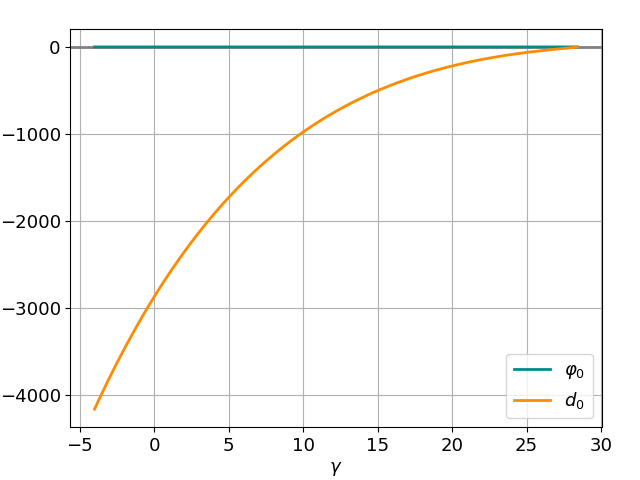
\includegraphics[scale=0.37]{oscillating_phi0d0_x0_067_beta_10.png} \\ {\scriptsize a) $ \beta = 1.0 $}
\end{center}
\end{minipage} 
\hfill
\begin{minipage}[h]{0.49\linewidth}
\begin{center}
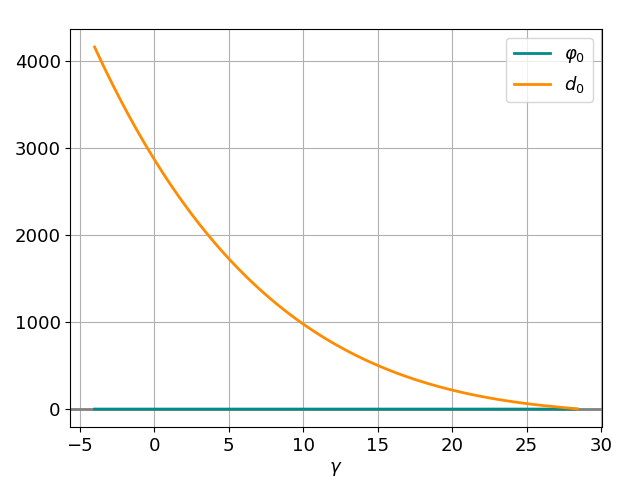
\includegraphics[scale=0.37]{oscillating_phi0d0_x0_067_beta_-10.png}  \\ {\scriptsize b) $ \beta = -1.0 $}
\end{center}
\end{minipage} 
\end{figure}
$$ \gamma_* \approx 28.407 $$

\end{frame}

\begin{frame}
\frametitle{ Plot $ \phi_0(\gamma) $ and $ d_0(\gamma), \; \alpha_{cr} = \alpha_f, k = 33 $ }

\begin{figure} 
\begin{minipage}[h]{0.49\linewidth}
\begin{center}
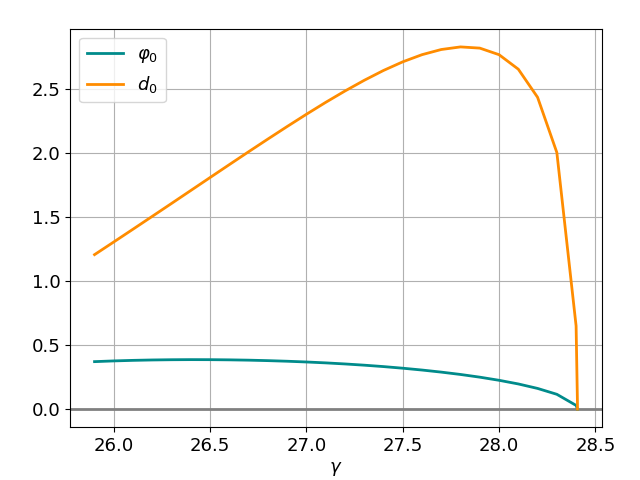
\includegraphics[scale=0.37]{oscillating_phi0d0_after_tangent_x0_067_beta_10.png} \\ {\scriptsize a) $ \beta = 1.0 $}
\end{center}
\end{minipage} 
\hfill
\begin{minipage}[h]{0.49\linewidth}
\begin{center}
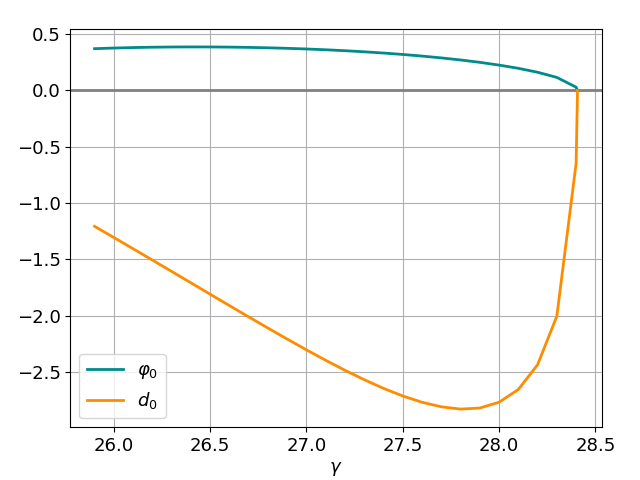
\includegraphics[scale=0.37]{oscillating_phi0d0_after_tangent_x0_067_beta_-10.png}  \\ {\scriptsize b) $ \beta = -1.0 $}
\end{center}
\end{minipage} 
\end{figure}
$$ \overline{\gamma} \approx 25.682, \; \gamma_* \approx 28.407 $$

\end{frame}

\begin{frame}
\titlepage
\end{frame}

\end{document}